% ═══════════════════════════════════════════════════════════════════════════════
% Chapter 5: Transformers and Large Language Models
% Part II: The Intelligence Stack
% ═══════════════════════════════════════════════════════════════════════════════

\chapter{Transformers and Large Language Models}
\label{ch:transformers-llms}

\chapterepigraph{Attention is all you need---but perhaps not all you want.}{After Vaswani et al., 2017}

\noindent
Chapter~\ref{ch:ml-foundations} established the foundational building blocks of machine learning: neural networks, optimization, embeddings, and evolutionary algorithms. This chapter focuses on the single most consequential architecture of the modern deep learning era: the \emph{transformer}. We trace its development from the attention mechanism through the scaling revolution to the emergent capabilities of large language models (LLMs), and close with a careful analysis of the transformer paradigm's structural limitations---limitations that motivate the DOGMA architecture introduced in Chapter~\ref{ch:dogma-architecture}.

The transformer is not merely one architecture among many. It is, at the time of writing, the computational substrate upon which virtually all frontier AI systems are built. Understanding it deeply---its mathematical structure, its scaling behavior, its surprising emergent properties, and its fundamental constraints---is prerequisite to understanding why DOGMA proposes a different organizational principle for intelligence.

This chapter is deliberately more detailed than a typical survey. We will work through every matrix multiplication, trace every gradient, and build intuition from concrete numerical examples. If you can reconstruct scaled dot-product attention on a napkin by the end of this chapter, you are ready for DOGMA.

% ───────────────────────────────────────────────────────────────────────────────
\section{The Attention Mechanism}
\label{sec:attention}

\subsection{From Alignment to Attention}

The attention mechanism was originally introduced for neural machine translation, where it allowed the decoder to dynamically focus on relevant parts of the source sentence rather than compressing the entire input into a fixed-length vector \citep{bahdanau2015}. The key insight: not all input positions are equally relevant to producing each output position, and the model should learn to \emph{selectively attend} to the most informative sources.

Consider translating the French sentence ``Le chat noir dort sur le tapis'' into English. When generating the word ``black,'' the model should focus on ``noir''; when generating ``sleeps,'' it should focus on ``dort.'' Before attention, sequence-to-sequence models compressed the entire source sentence into a single fixed-length vector, forcing all information through a bottleneck. Attention removes this bottleneck by allowing the decoder to look back at the full source sequence at every generation step.

\begin{bioinsight}[Attention and Transcription Factor Binding]
Biological transcription factors selectively bind to specific promoter and enhancer regions, activating only the relevant genes for a given cellular context. Attention performs an analogous function: given a query (the current context), it selectively weights source positions (the ``genome'' of input tokens) to determine which information flows forward. DOGMA's regulation stage (Chapter~\ref{ch:dogma-architecture}) generalizes this idea beyond pairwise token comparisons to typed, region-level regulatory control.
\end{bioinsight}

\subsection{Intuition: Queries, Keys, and Values}
\label{sec:qkv-intuition}

Before diving into the mathematics, let us build intuition for the three central objects in attention: \textbf{queries}, \textbf{keys}, and \textbf{values}. The analogy to a database lookup is instructive:

\begin{itemize}[leftmargin=1.5em]
  \item \textbf{Query ($\mathbf{Q}$):} ``What am I looking for?'' Each token produces a query vector that encodes what information it needs from other tokens. Think of it as a search query in a database.
  \item \textbf{Key ($\mathbf{K}$):} ``What do I contain?'' Each token also produces a key vector that advertises what information it has available. Think of it as the index entry in a database.
  \item \textbf{Value ($\mathbf{V}$):} ``What do I actually return?'' Each token produces a value vector that is the content to be retrieved. Think of it as the data record that the index points to.
\end{itemize}

The attention mechanism computes a \emph{soft lookup}: each query is compared against all keys to produce a relevance score, and the output is a weighted combination of values, where the weights are proportional to the relevance scores. Unlike a hard database lookup that returns a single record, attention returns a blended combination of all records, weighted by relevance.

\begin{remark}
The query, key, and value vectors are \emph{all derived from the same input} in self-attention. Each token simultaneously asks a question (query), advertises its content (key), and provides retrievable information (value). The three roles are distinguished only by the learned projection matrices $\mathbf{W}_Q$, $\mathbf{W}_K$, and $\mathbf{W}_V$.
\end{remark}

\subsection{Scaled Dot-Product Attention}

The transformer's attention mechanism operates on three learned projections of the input: \emph{queries} $\mathbf{Q}$, \emph{keys} $\mathbf{K}$, and \emph{values} $\mathbf{V}$. Given an input matrix $\mathbf{X} \in \mathbb{R}^{T \times d}$ representing $T$ tokens of dimension $d$, these projections are:

\begin{equation}
\mathbf{Q} = \mathbf{X}\mathbf{W}_Q, \quad
\mathbf{K} = \mathbf{X}\mathbf{W}_K, \quad
\mathbf{V} = \mathbf{X}\mathbf{W}_V,
\label{eq:qkv}
\end{equation}

where $\mathbf{W}_Q, \mathbf{W}_K \in \mathbb{R}^{d \times d_k}$ and $\mathbf{W}_V \in \mathbb{R}^{d \times d_v}$ are learned parameter matrices. Scaled dot-product attention then computes:

\begin{equation}
\text{Attention}(\mathbf{Q}, \mathbf{K}, \mathbf{V}) = \operatorname{softmax}\!\left(\frac{\mathbf{Q}\mathbf{K}^\top}{\sqrt{d_k}}\right)\mathbf{V}.
\label{eq:scaled-attention}
\end{equation}

Let us break this computation into four explicit steps:

\begin{enumerate}[leftmargin=1.8em]
  \item \textbf{Compute raw attention scores:} $\mathbf{S} = \mathbf{Q}\mathbf{K}^\top \in \mathbb{R}^{T \times T}$. Entry $S_{ij}$ measures how much token $i$'s query aligns with token $j$'s key---i.e., how relevant token $j$'s content is to token $i$'s current need.
  \item \textbf{Scale:} $\mathbf{S}' = \mathbf{S} / \sqrt{d_k}$. Without scaling, the dot products grow in magnitude proportionally to $d_k$ (since each is a sum of $d_k$ terms). Large magnitudes push the softmax into saturated regions where gradients vanish. Dividing by $\sqrt{d_k}$ keeps the variance of the scores approximately 1, regardless of the dimension.
  \item \textbf{Normalize with softmax:} $\mathbf{A} = \operatorname{softmax}(\mathbf{S}')$, applied row-wise. Each row of $\mathbf{A}$ is a probability distribution over all tokens, with $A_{ij} \geq 0$ and $\sum_j A_{ij} = 1$. This converts raw scores into normalized attention weights.
  \item \textbf{Aggregate values:} $\mathbf{O} = \mathbf{A}\mathbf{V} \in \mathbb{R}^{T \times d_v}$. The output for token $i$ is a weighted average of all value vectors: $\mathbf{o}_i = \sum_j A_{ij} \mathbf{v}_j$.
\end{enumerate}

\begin{dogmadef}[Attention Complexity]
The attention matrix $\mathbf{A} = \operatorname{softmax}(\mathbf{Q}\mathbf{K}^\top / \sqrt{d_k})$ has shape $T \times T$, making the time and space complexity of self-attention $O(T^2 \cdot d_k)$. For a sequence of length $T = 128{,}000$ tokens with $d_k = 128$, the attention matrix alone contains $\approx 1.6 \times 10^{10}$ entries---a fundamental bottleneck that limits the transformer's ability to process long sequences efficiently.
\end{dogmadef}

\subsection{Why the Scaling Factor Matters}

To understand the scaling factor $1/\sqrt{d_k}$ more concretely, suppose the entries of $\mathbf{q}$ and $\mathbf{k}$ are independent random variables with mean 0 and variance 1. Then the dot product $\mathbf{q} \cdot \mathbf{k} = \sum_{j=1}^{d_k} q_j k_j$ has mean 0 and variance $d_k$ (since each product $q_j k_j$ contributes variance 1, and the terms are independent). For $d_k = 64$, the standard deviation of $\mathbf{q} \cdot \mathbf{k}$ is $\sqrt{64} = 8$. Dot products of magnitude 8 or larger push softmax outputs toward 0 or 1, creating nearly one-hot attention patterns that produce vanishingly small gradients. Dividing by $\sqrt{d_k} = 8$ rescales the standard deviation back to 1, keeping softmax in a well-behaved regime.

\subsection{Worked Example: Self-Attention with 3 Tokens}
\label{sec:attention-worked-example}

Let us trace through a complete self-attention computation with $T = 3$ tokens and $d_k = d_v = 4$. Suppose after the linear projections, we have:

\begin{equation}
\mathbf{Q} = \begin{pmatrix} 1 & 0 & 1 & 0 \\ 0 & 1 & 0 & 1 \\ 1 & 1 & 0 & 0 \end{pmatrix}, \quad
\mathbf{K} = \begin{pmatrix} 0 & 1 & 1 & 0 \\ 1 & 0 & 0 & 1 \\ 1 & 1 & 0 & 0 \end{pmatrix}, \quad
\mathbf{V} = \begin{pmatrix} 1 & 2 & 3 & 4 \\ 5 & 6 & 7 & 8 \\ 9 & 10 & 11 & 12 \end{pmatrix}.
\end{equation}

\textbf{Step 1: Raw attention scores.} Compute $\mathbf{S} = \mathbf{Q}\mathbf{K}^\top$:

\begin{equation}
\mathbf{S} = \begin{pmatrix}
\mathbf{q}_1 \cdot \mathbf{k}_1 & \mathbf{q}_1 \cdot \mathbf{k}_2 & \mathbf{q}_1 \cdot \mathbf{k}_3 \\
\mathbf{q}_2 \cdot \mathbf{k}_1 & \mathbf{q}_2 \cdot \mathbf{k}_2 & \mathbf{q}_2 \cdot \mathbf{k}_3 \\
\mathbf{q}_3 \cdot \mathbf{k}_1 & \mathbf{q}_3 \cdot \mathbf{k}_2 & \mathbf{q}_3 \cdot \mathbf{k}_3
\end{pmatrix} = \begin{pmatrix}
1 & 1 & 1 \\
1 & 1 & 1 \\
1 & 1 & 2
\end{pmatrix}.
\end{equation}

For example, $S_{11} = (1)(0) + (0)(1) + (1)(1) + (0)(0) = 1$, and $S_{33} = (1)(1) + (1)(1) + (0)(0) + (0)(0) = 2$.

\textbf{Step 2: Scale.} With $d_k = 4$, we divide by $\sqrt{4} = 2$:

\begin{equation}
\mathbf{S}' = \frac{\mathbf{S}}{\sqrt{d_k}} = \begin{pmatrix} 0.5 & 0.5 & 0.5 \\ 0.5 & 0.5 & 0.5 \\ 0.5 & 0.5 & 1.0 \end{pmatrix}.
\end{equation}

\textbf{Step 3: Softmax (row-wise).} For rows 1 and 2, all entries are equal ($0.5$), so softmax gives uniform weights: $A_{1j} = A_{2j} = 1/3$ for all $j$. For row 3:

\begin{equation}
A_{31} = A_{32} = \frac{e^{0.5}}{2e^{0.5} + e^{1.0}} \approx \frac{1.649}{3.298 + 2.718} \approx 0.274, \quad
A_{33} = \frac{e^{1.0}}{2e^{0.5} + e^{1.0}} \approx \frac{2.718}{6.016} \approx 0.452.
\end{equation}

The full attention matrix is:
\begin{equation}
\mathbf{A} \approx \begin{pmatrix} 0.333 & 0.333 & 0.333 \\ 0.333 & 0.333 & 0.333 \\ 0.274 & 0.274 & 0.452 \end{pmatrix}.
\end{equation}

\textbf{Step 4: Weighted value aggregation.} The output $\mathbf{O} = \mathbf{A}\mathbf{V}$:

\begin{equation}
\mathbf{o}_1 = 0.333 \cdot \begin{pmatrix}1\\2\\3\\4\end{pmatrix} + 0.333 \cdot \begin{pmatrix}5\\6\\7\\8\end{pmatrix} + 0.333 \cdot \begin{pmatrix}9\\10\\11\\12\end{pmatrix} = \begin{pmatrix}5.0\\6.0\\7.0\\8.0\end{pmatrix}.
\end{equation}

Token 1 attends uniformly, so its output is the average of all value vectors. Token 3, however, attends more heavily to itself (weight 0.452 vs.\ 0.274), so its output is shifted toward $\mathbf{v}_3$:

\begin{equation}
\mathbf{o}_3 \approx 0.274 \cdot \begin{pmatrix}1\\2\\3\\4\end{pmatrix} + 0.274 \cdot \begin{pmatrix}5\\6\\7\\8\end{pmatrix} + 0.452 \cdot \begin{pmatrix}9\\10\\11\\12\end{pmatrix} \approx \begin{pmatrix}5.70\\6.70\\7.70\\8.70\end{pmatrix}.
\end{equation}

\begin{example}[Interpreting Attention Weights]
In the worked example above, tokens 1 and 2 attend uniformly to all tokens---they have no strong preference. Token 3 attends preferentially to itself because $\mathbf{q}_3 \cdot \mathbf{k}_3 = 2 > 1 = \mathbf{q}_3 \cdot \mathbf{k}_j$ for $j \neq 3$. In practice, attention heads learn to produce query-key alignments that reflect semantic relationships: a pronoun's query might strongly match the key of its antecedent, producing a high attention weight that copies the antecedent's information into the pronoun's representation.
\end{example}

\subsection{Visualizing Self-Attention}

Figure~\ref{fig:attention-mechanism} illustrates the self-attention mechanism with colored arrows showing how tokens selectively attend to each other.

\begin{figure}[ht]
\centering
\begin{tikzpicture}[
  token/.style={draw, rounded corners=3pt, minimum width=1.2cm, minimum height=0.6cm, font=\small\bfseries, fill=dogmalight},
  qbox/.style={draw, rounded corners=2pt, minimum width=0.8cm, minimum height=0.5cm, font=\scriptsize, fill=blue!10},
  kbox/.style={draw, rounded corners=2pt, minimum width=0.8cm, minimum height=0.5cm, font=\scriptsize, fill=red!10},
  vbox/.style={draw, rounded corners=2pt, minimum width=0.8cm, minimum height=0.5cm, font=\scriptsize, fill=green!10},
  outbox/.style={draw, rounded corners=2pt, minimum width=0.8cm, minimum height=0.5cm, font=\scriptsize, fill=orange!10},
  proj/.style={->, >=stealth, thick},
  attn/.style={->, >=stealth, thick, dogmablue, opacity=0.6},
  attnh/.style={->, >=stealth, very thick, dogmared, opacity=0.8},
]
  % Input tokens
  \node[token] (t1) at (0, 0) {The};
  \node[token] (t2) at (2.5, 0) {cat};
  \node[token] (t3) at (5.0, 0) {sat};

  % Q, K, V projections
  \node[qbox] (q1) at (-0.8, 1.5) {$\mathbf{q}_1$};
  \node[kbox] (k1) at (0.0, 1.5) {$\mathbf{k}_1$};
  \node[vbox] (v1) at (0.8, 1.5) {$\mathbf{v}_1$};

  \node[qbox] (q2) at (1.7, 1.5) {$\mathbf{q}_2$};
  \node[kbox] (k2) at (2.5, 1.5) {$\mathbf{k}_2$};
  \node[vbox] (v2) at (3.3, 1.5) {$\mathbf{v}_2$};

  \node[qbox] (q3) at (4.2, 1.5) {$\mathbf{q}_3$};
  \node[kbox] (k3) at (5.0, 1.5) {$\mathbf{k}_3$};
  \node[vbox] (v3) at (5.8, 1.5) {$\mathbf{v}_3$};

  % Projections from tokens
  \draw[proj] (t1.north) -- (q1.south);
  \draw[proj] (t1.north) -- (k1.south);
  \draw[proj] (t1.north) -- (v1.south);
  \draw[proj] (t2.north) -- (q2.south);
  \draw[proj] (t2.north) -- (k2.south);
  \draw[proj] (t2.north) -- (v2.south);
  \draw[proj] (t3.north) -- (q3.south);
  \draw[proj] (t3.north) -- (k3.south);
  \draw[proj] (t3.north) -- (v3.south);

  % Attention computation label
  \node[font=\small, align=center] at (2.5, 3.0) {$\operatorname{softmax}\!\left(\frac{\mathbf{Q}\mathbf{K}^\top}{\sqrt{d_k}}\right)\mathbf{V}$};

  % Output tokens
  \node[outbox] (o1) at (0, 4.2) {$\mathbf{o}_1$};
  \node[outbox] (o2) at (2.5, 4.2) {$\mathbf{o}_2$};
  \node[outbox] (o3) at (5.0, 4.2) {$\mathbf{o}_3$};

  % Attention arrows (showing that token 3 "sat" attends heavily to token 2 "cat")
  \draw[attn] (v1.north) to[bend left=15] (o1.south);
  \draw[attn] (v2.north) to[bend left=5] (o1.south);
  \draw[attn] (v3.north) to[bend right=15] (o1.south);

  \draw[attn] (v1.north) to[bend left=15] (o2.south);
  \draw[attnh] (v2.north) to[bend left=5] (o2.south);
  \draw[attn] (v3.north) to[bend right=15] (o2.south);

  \draw[attn] (v1.north) to[bend left=15] (o3.south);
  \draw[attnh] (v2.north) to[bend left=5] (o3.south);
  \draw[attnh] (v3.north) to[bend right=5] (o3.south);

  % Legend
  \node[font=\scriptsize, dogmablue] at (8.0, 4.2) {Low attention};
  \draw[attn] (6.5, 4.2) -- (7.0, 4.2);
  \node[font=\scriptsize, dogmared] at (8.0, 3.7) {High attention};
  \draw[attnh] (6.5, 3.7) -- (7.0, 3.7);
\end{tikzpicture}
\caption{Self-attention mechanism for three tokens. Each token is projected into query ($\mathbf{q}$), key ($\mathbf{k}$), and value ($\mathbf{v}$) vectors. Attention scores (computed as $\mathbf{q}_i \cdot \mathbf{k}_j / \sqrt{d_k}$, then softmax-normalized) determine how much of each value vector contributes to each output. Thicker red arrows indicate higher attention weights.}
\label{fig:attention-mechanism}
\end{figure}

% ───────────────────────────────────────────────────────────────────────────────
\section{Multi-Head Attention}
\label{sec:multihead-attention}

\subsection{Why Multiple Heads?}

A single attention head computes a single set of attention weights for each pair of tokens. But different aspects of the relationship between two tokens may be relevant simultaneously. For instance, when processing the sentence ``The animal didn't cross the street because it was too tired,'' one attention head might need to resolve the pronoun ``it'' (a syntactic task), while another might need to capture the semantic relationship between ``tired'' and ``animal'' (a semantic task). A single head must compress all of these relationships into one set of weights---an information bottleneck.

\emph{Multi-head attention} solves this by running $h$ independent attention computations in parallel, each with its own learned projections:

\begin{equation}
\text{MultiHead}(\mathbf{Q}, \mathbf{K}, \mathbf{V}) = \operatorname{Concat}(\text{head}_1, \ldots, \text{head}_h)\,\mathbf{W}_O,
\label{eq:multihead}
\end{equation}

where each head is:
\begin{equation}
\text{head}_i = \text{Attention}(\mathbf{X}\mathbf{W}_Q^{(i)},\; \mathbf{X}\mathbf{W}_K^{(i)},\; \mathbf{X}\mathbf{W}_V^{(i)}),
\end{equation}

and $\mathbf{W}_O \in \mathbb{R}^{hd_v \times d}$ is a learned output projection.

\subsection{Head Splitting and Concatenation}

In practice, multi-head attention does \emph{not} require $h$ separate sets of full-sized projection matrices. Instead, the model dimension $d$ is split evenly across the $h$ heads: each head operates on $d_k = d_v = d / h$ dimensions. This means:

\begin{itemize}[leftmargin=1.5em]
  \item $\mathbf{W}_Q^{(i)}, \mathbf{W}_K^{(i)} \in \mathbb{R}^{d \times (d/h)}$ --- each head projects from the full $d$-dimensional space into a $(d/h)$-dimensional subspace.
  \item Each head independently computes attention in its $(d/h)$-dimensional subspace, producing output of shape $T \times (d/h)$.
  \item The $h$ head outputs are concatenated along the feature dimension, giving shape $T \times d$.
  \item The concatenated output is projected through $\mathbf{W}_O \in \mathbb{R}^{d \times d}$ to produce the final output.
\end{itemize}

The total number of parameters is the same as a single head with $d_k = d$: the computation is \emph{repartitioned}, not increased. With $h = 12$ heads and $d = 768$ (as in BERT-base), each head operates on $d_k = 64$ dimensions.

\subsection{What Different Heads Learn}

Empirical analysis reveals that attention heads specialize in different linguistic functions \citep{voita2019}:

\begin{itemize}[leftmargin=1.5em]
  \item \textbf{Positional heads:} Attend to the immediately preceding or following token---capturing local context.
  \item \textbf{Syntactic heads:} Attend to syntactically related tokens (e.g., a verb head attends to its subject).
  \item \textbf{Rare-word heads:} Attend to the least frequent token in the sequence---potentially copying specialized information.
  \item \textbf{Delimiter heads:} Attend to separator tokens (periods, commas)---capturing sentence boundaries.
\end{itemize}

This emergent specialization occurs without any explicit supervision: the heads discover useful attention patterns through gradient descent alone.

\subsection{Multi-Head Attention Diagram}

\begin{figure}[ht]
\centering
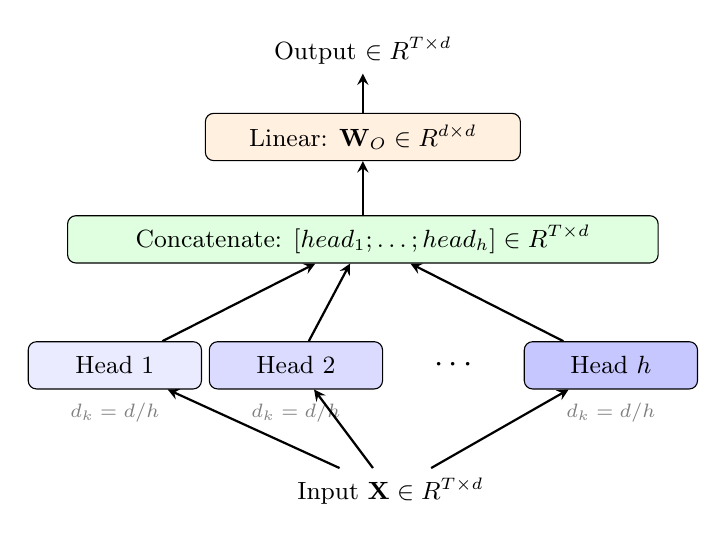
\begin{tikzpicture}[
  block/.style={draw, rounded corners=3pt, minimum width=2.2cm, minimum height=0.6cm, align=center, font=\small},
  arr/.style={->, >=stealth, thick},
]
  % Input
  \node (input) at (0, 0) {\small Input $\mathbf{X} \in \mathbb{R}^{T \times d}$};

  % Heads
  \node[block, fill=blue!8] (h1) at (-3.5, 1.6) {Head 1};
  \node[block, fill=blue!14] (h2) at (-1.2, 1.6) {Head 2};
  \node[font=\large] at (0.8, 1.6) {$\cdots$};
  \node[block, fill=blue!22] (hh) at (2.8, 1.6) {Head $h$};

  % Internal labels
  \node[font=\scriptsize, gray] at (-3.5, 1.0) {$d_k = d/h$};
  \node[font=\scriptsize, gray] at (-1.2, 1.0) {$d_k = d/h$};
  \node[font=\scriptsize, gray] at (2.8, 1.0) {$d_k = d/h$};

  % Concat
  \node[block, fill=green!12, minimum width=7.5cm] (concat) at (-0.35, 3.2) {Concatenate: $[\text{head}_1; \ldots; \text{head}_h] \in \mathbb{R}^{T \times d}$};

  % Output projection
  \node[block, fill=orange!12, minimum width=4.0cm] (proj) at (-0.35, 4.5) {Linear: $\mathbf{W}_O \in \mathbb{R}^{d \times d}$};

  % Output
  \node (output) at (-0.35, 5.6) {\small Output $\in \mathbb{R}^{T \times d}$};

  % Arrows
  \draw[arr] (input) -- (h1);
  \draw[arr] (input) -- (h2);
  \draw[arr] (input) -- (hh);
  \draw[arr] (h1) -- (concat);
  \draw[arr] (h2) -- (concat);
  \draw[arr] (hh) -- (concat);
  \draw[arr] (concat) -- (proj);
  \draw[arr] (proj) -- (output);
\end{tikzpicture}
\caption{Multi-head attention. The input is processed by $h$ independent attention heads, each operating in a $(d/h)$-dimensional subspace. Outputs are concatenated and projected back to the full $d$-dimensional space.}
\label{fig:multihead-attention}
\end{figure}

% ───────────────────────────────────────────────────────────────────────────────
\section{The Transformer Architecture}
\label{sec:transformer-arch}

\citet{vaswani2017} introduced the transformer as a sequence-to-sequence architecture composed entirely of attention and feedforward layers, eliminating the recurrence that had characterized prior sequence models. The architecture consists of an \emph{encoder} stack and a \emph{decoder} stack, each built from repeated identical layers.

\subsection{Encoder and Decoder Stacks}

Each encoder layer applies two sub-layers:
\begin{enumerate}[leftmargin=1.8em]
  \item \textbf{Multi-head self-attention:} Each position attends to all positions in the input.
  \item \textbf{Position-wise feedforward network (FFN):} A two-layer MLP applied independently to each position:
  \begin{equation}
    \text{FFN}(\mathbf{x}) = \text{ReLU}(\mathbf{x}\mathbf{W}_1 + \mathbf{b}_1)\mathbf{W}_2 + \mathbf{b}_2.
    \label{eq:ffn}
  \end{equation}
\end{enumerate}

The FFN is a critical but often underappreciated component. While attention handles \emph{inter-token} communication (allowing tokens to share information), the FFN handles \emph{intra-token} processing (transforming each token's representation independently). In GPT-3, the FFN inner dimension is $4d = 49{,}152$ for $d = 12{,}288$---meaning the FFN has $4 \times$ the width of the model dimension. Research suggests that FFN layers function as key-value memories, storing factual associations learned during training.

Each decoder layer adds a third sub-layer: \emph{cross-attention} over the encoder output, allowing the decoder to condition on the full input sequence while generating the output autoregressively.

\subsection{Residual Connections and Layer Normalization}

Both encoder and decoder employ \emph{residual connections} \citep{he2016} around each sub-layer, followed by \emph{layer normalization} \citep{ba2016}:

\begin{equation}
\mathbf{y} = \text{LayerNorm}(\mathbf{x} + \text{SubLayer}(\mathbf{x})).
\label{eq:residual-ln}
\end{equation}

\textbf{Residual connections} add the sub-layer's input directly to its output: $\mathbf{x} + \text{SubLayer}(\mathbf{x})$. This creates a ``skip connection'' that allows gradients to flow directly through the network without passing through every sub-layer. Without residual connections, training transformers with $L > 6$ layers would be extremely difficult due to vanishing or exploding gradients.

\textbf{Layer normalization} normalizes activations across the feature dimension for each token independently. Given a vector $\mathbf{x} \in \mathbb{R}^d$:

\begin{equation}
\text{LayerNorm}(\mathbf{x}) = \gamma \odot \frac{\mathbf{x} - \mu}{\sigma + \epsilon} + \beta,
\label{eq:layernorm}
\end{equation}

where $\mu = \frac{1}{d}\sum_{i=1}^{d} x_i$, $\sigma = \sqrt{\frac{1}{d}\sum_{i=1}^{d}(x_i - \mu)^2}$, and $\gamma, \beta \in \mathbb{R}^d$ are learned scale and shift parameters. The small constant $\epsilon$ (typically $10^{-5}$) prevents division by zero.

Modern implementations often use \emph{pre-norm} placement, applying normalization before the sub-layer rather than after:

\begin{equation}
\mathbf{y} = \mathbf{x} + \text{SubLayer}(\text{LayerNorm}(\mathbf{x})),
\label{eq:pre-norm}
\end{equation}

which improves training stability for very deep models. Pre-norm is now standard in models like GPT-3, LLaMA, and their descendants.

\subsection{The Complete Transformer Block}

Figure~\ref{fig:transformer-block} illustrates the structure of a single transformer decoder block with all components labeled.

\begin{figure}[ht]
\centering
\begin{tikzpicture}[
  block/.style={draw, rounded corners=3pt, minimum width=5.2cm, minimum height=0.7cm, align=center, font=\small},
  addnorm/.style={draw, rounded corners=3pt, minimum width=5.2cm, minimum height=0.55cm, fill=gray!12, align=center, font=\small},
  normblock/.style={draw, rounded corners=3pt, minimum width=5.2cm, minimum height=0.55cm, fill=dogmamint!40, align=center, font=\small},
  arr/.style={->, >=stealth, thick},
  skip/.style={->, >=stealth, thick, dashed, gray},
  annot/.style={font=\scriptsize, text=dogmagold, align=left},
]
  % Input
  \node (input) at (0, 0) {\small Input Embeddings $+ \text{PE}$};

  % Pre-norm 1
  \node[normblock] (ln1) at (0, 1.0) {LayerNorm};

  % Masked Multi-Head Attention
  \node[block, fill=blue!12] (mha) at (0, 2.2) {Masked Multi-Head Attention};

  % Add
  \node[addnorm] (add1) at (0, 3.2) {Add (Residual)};

  % Pre-norm 2
  \node[normblock] (ln2) at (0, 4.2) {LayerNorm};

  % FFN
  \node[block, fill=orange!15] (ffn) at (0, 5.4) {Feed-Forward Network};

  % Add
  \node[addnorm] (add2) at (0, 6.4) {Add (Residual)};

  % Output
  \node (output) at (0, 7.4) {\small To Next Layer};

  % Vertical arrows
  \draw[arr] (input) -- (ln1);
  \draw[arr] (ln1) -- (mha);
  \draw[arr] (mha) -- (add1);
  \draw[arr] (add1) -- (ln2);
  \draw[arr] (ln2) -- (ffn);
  \draw[arr] (ffn) -- (add2);
  \draw[arr] (add2) -- (output);

  % Residual connections
  \draw[skip] (input.east) -- ++(1.8,0) |- ([yshift=-2mm]add1.east);
  \draw[skip] (add1.east) -- ++(1.6,0) |- (add2.east);

  % Labels for residual
  \node[font=\scriptsize, gray] at (3.0, 1.6) {residual};
  \node[font=\scriptsize, gray] at (3.3, 4.8) {residual};

  % Annotations
  \node[annot, anchor=west] at (4.0, 2.2) {$h$ parallel heads\\each $d_k = d/h$};
  \node[annot, anchor=west] at (4.2, 5.4) {$\text{ReLU}(\mathbf{x}\mathbf{W}_1\!+\!\mathbf{b}_1)\mathbf{W}_2\!+\!\mathbf{b}_2$\\inner dim $= 4d$};

  % N times bracket
  \draw[decorate, decoration={brace, amplitude=6pt, mirror}, thick] (-3.4, 0.6) -- (-3.4, 6.8);
  \node[font=\small, rotate=90] at (-4.1, 3.7) {$\times\, L$ layers};
\end{tikzpicture}
\caption{A single transformer decoder block with pre-norm residual connections. The masked multi-head attention sub-layer prevents each position from attending to future tokens. LayerNorm is applied before each sub-layer (pre-norm configuration). The block is repeated $L$ times to form the full decoder stack.}
\label{fig:transformer-block}
\end{figure}

% ───────────────────────────────────────────────────────────────────────────────
\section{Positional Encoding}
\label{sec:positional-encoding}

\subsection{The Permutation Equivariance Problem}

Self-attention is \emph{permutation equivariant}: if we shuffle the order of input tokens, the output is shuffled in exactly the same way. Mathematically, for any permutation matrix $\mathbf{P}$:

\begin{equation}
\text{Attention}(\mathbf{P}\mathbf{Q}, \mathbf{P}\mathbf{K}, \mathbf{P}\mathbf{V}) = \mathbf{P} \cdot \text{Attention}(\mathbf{Q}, \mathbf{K}, \mathbf{V}).
\end{equation}

This means that without additional information, the transformer treats ``The cat sat'' and ``sat cat The'' identically. Since word order is essential for meaning, positional information must be injected explicitly.

\subsection{Sinusoidal Positional Encodings}

\citet{vaswani2017} proposed sinusoidal positional encodings, where each position $t$ and dimension $i$ receives a unique value:

\begin{align}
\text{PE}(t, 2i) &= \sin\!\left(\frac{t}{10000^{2i/d}}\right), \label{eq:pe-sin} \\
\text{PE}(t, 2i+1) &= \cos\!\left(\frac{t}{10000^{2i/d}}\right). \label{eq:pe-cos}
\end{align}

These encodings are added to the input embeddings: $\mathbf{x}_t' = \mathbf{x}_t + \text{PE}(t)$.

\textbf{Why sinusoids?} The key property is that relative positions can be computed as linear transformations. For any fixed offset $k$, there exists a matrix $\mathbf{M}_k$ (independent of position $t$) such that $\text{PE}(t+k) = \mathbf{M}_k \cdot \text{PE}(t)$. This follows from the trigonometric identity $\sin(\alpha + \beta) = \sin\alpha\cos\beta + \cos\alpha\sin\beta$. The model can therefore learn to attend to relative positions (e.g., ``the token 3 positions back'') using fixed linear operations, without needing to memorize absolute positions.

\textbf{Multi-frequency structure.} Different dimensions encode position at different frequencies. Low dimensions ($i \approx 0$) use high frequencies (fast oscillation), capturing fine-grained positional differences. High dimensions ($i \approx d/2$) use low frequencies (slow oscillation), capturing long-range positional structure. The model has access to a rich, multi-scale representation of position.

\begin{example}[Positional Encoding Values]
For $d = 4$, the positional encoding at position $t$ is a 4-dimensional vector:
\begin{equation}
\text{PE}(t) = \begin{pmatrix}
\sin(t / 10000^{0/4}) \\
\cos(t / 10000^{0/4}) \\
\sin(t / 10000^{2/4}) \\
\cos(t / 10000^{2/4})
\end{pmatrix} = \begin{pmatrix}
\sin(t) \\
\cos(t) \\
\sin(t/100) \\
\cos(t/100)
\end{pmatrix}.
\end{equation}
Dimension 0 oscillates rapidly (period $2\pi \approx 6.3$ positions), while dimension 2 oscillates slowly (period $200\pi \approx 628$ positions). At position $t=0$: $\text{PE}(0) = (0, 1, 0, 1)^\top$. At position $t=1$: $\text{PE}(1) \approx (0.841, 0.540, 0.010, 1.000)^\top$.
\end{example}

\subsection{Learned and Relative Position Encodings}

\textbf{Learned positional embeddings.} An alternative is to learn a separate embedding vector for each position, stored as a matrix $\mathbf{E}_{\text{pos}} \in \mathbb{R}^{T_{\max} \times d}$. GPT-2 and BERT use this approach. The downside: the model cannot generalize to positions beyond $T_{\max}$.

\textbf{Rotary Position Embeddings (RoPE).} Modern models commonly use RoPE \citep{su2024}, which encode relative distances through rotation matrices applied to query and key vectors. RoPE rotates pairs of dimensions by an angle proportional to position:

\begin{equation}
\text{RoPE}(\mathbf{x}_t, t) = \begin{pmatrix}
x_1 \cos(t\theta_1) - x_2 \sin(t\theta_1) \\
x_1 \sin(t\theta_1) + x_2 \cos(t\theta_1) \\
\vdots \\
x_{d-1} \cos(t\theta_{d/2}) - x_d \sin(t\theta_{d/2}) \\
x_{d-1} \sin(t\theta_{d/2}) + x_d \cos(t\theta_{d/2})
\end{pmatrix},
\label{eq:rope}
\end{equation}

where $\theta_i = 10000^{-2i/d}$. The key property is that the dot product $\text{RoPE}(\mathbf{q}_m, m)^\top \text{RoPE}(\mathbf{k}_n, n)$ depends only on $\mathbf{q}_m$, $\mathbf{k}_n$, and the \emph{relative position} $m - n$, not on the absolute positions $m$ and $n$. This enables length generalization: models trained with RoPE can often handle sequences longer than those seen during training.

% ───────────────────────────────────────────────────────────────────────────────
\section{GPT and Autoregressive Language Models}
\label{sec:gpt}

\subsection{Decoder-Only Architecture}

While the original transformer used both encoder and decoder stacks, the GPT family \citep{radford2019} demonstrated that a \emph{decoder-only} architecture---using only the masked self-attention stack---is sufficient for powerful language modeling. The key simplification: by training the model to predict the next token given all preceding tokens, the encoder becomes unnecessary.

A decoder-only model with parameters $\theta$ defines a probability distribution over sequences:

\begin{equation}
p_\theta(x_1, x_2, \ldots, x_T) = \prod_{t=1}^{T} p_\theta(x_t \mid x_1, \ldots, x_{t-1}).
\label{eq:autoregressive}
\end{equation}

This factorization is exact by the chain rule of probability. The model is trained by maximizing the log-likelihood of the training corpus, which is equivalent to minimizing the cross-entropy loss introduced in Equation~\ref{eq:lm-loss} of Chapter~\ref{ch:ml-foundations}.

\subsection{The Next-Token Prediction Objective}
\label{sec:next-token}

The training objective for autoregressive language models is deceptively simple: predict the next token. Given a sequence of tokens $(x_1, x_2, \ldots, x_T)$ from the training corpus, the cross-entropy loss is:

\begin{equation}
\mathcal{L}(\theta) = -\frac{1}{T}\sum_{t=1}^{T} \log p_\theta(x_t \mid x_1, \ldots, x_{t-1}).
\label{eq:lm-cross-entropy}
\end{equation}

At each position $t$, the model produces a probability distribution over the entire vocabulary $\mathcal{V}$ (typically 32,000 to 128,000 tokens). The loss penalizes the model for assigning low probability to the actual next token. Minimizing this loss across trillions of tokens forces the model to develop rich internal representations of language, world knowledge, and reasoning patterns.

\begin{example}[Cross-Entropy Loss Computation]
Suppose the vocabulary is $\mathcal{V} = \{\texttt{the}, \texttt{cat}, \texttt{sat}, \texttt{on}\}$ and we are predicting position 3 given ``The cat \underline{\phantom{sat}}''. If the model assigns probabilities $(0.05, 0.10, 0.80, 0.05)$ to the four tokens, the loss for this position is:
\begin{equation}
\mathcal{L}_3 = -\log p(\texttt{sat}) = -\log(0.80) \approx 0.223.
\end{equation}
If the model were less confident and assigned $p(\texttt{sat}) = 0.25$, the loss would be $-\log(0.25) \approx 1.386$---much higher. The loss is minimized (to zero) only when the model assigns probability 1 to the correct next token.
\end{example}

\subsection{Causal Masking}

To enforce the autoregressive property during training, a \emph{causal mask} $\mathbf{M}$ is applied to the attention scores before the softmax:

\begin{equation}
\mathbf{A} = \operatorname{softmax}\!\left(\frac{\mathbf{Q}\mathbf{K}^\top}{\sqrt{d_k}} + \mathbf{M}\right), \quad M_{ij} = \begin{cases} 0 & \text{if } i \geq j, \\ -\infty & \text{if } i < j. \end{cases}
\label{eq:causal-mask}
\end{equation}

This ensures that position $i$ can only attend to positions $j \leq i$, preventing information leakage from future tokens. Causal masking enables efficient training: the entire sequence can be processed in a single forward pass, with losses computed at every position simultaneously (teacher forcing).

\begin{keyinsight}[Causal Masking vs.\ Biological Directionality]
DNA transcription proceeds in the $5' \to 3'$ direction, and ribosomes translate mRNA codons sequentially from start to stop. There is a natural directionality to biological information flow. Causal masking in autoregressive models enforces a similar sequential constraint. However, biological systems also permit \emph{bidirectional} regulatory signals: enhancers can act upstream or downstream of their target genes, and chromatin loops bring distant regulatory elements into spatial proximity. DOGMA's regulation stage captures this bidirectional control while maintaining directionality in the transcription and expression stages.
\end{keyinsight}

% ───────────────────────────────────────────────────────────────────────────────
\section{Training Large Language Models}
\label{sec:training-llms}

\subsection{Training Data Scale}

Modern LLMs are trained on colossal datasets. The training corpus for a frontier model typically includes:

\begin{itemize}[leftmargin=1.5em]
  \item \textbf{Web text:} Crawled and filtered web pages (Common Crawl, typically 1--5 trillion tokens after filtering).
  \item \textbf{Books:} Digitized books providing long-form, high-quality prose.
  \item \textbf{Code:} Source code from public repositories (GitHub), which improves reasoning abilities.
  \item \textbf{Scientific papers:} ArXiv, PubMed, and other academic sources.
  \item \textbf{Conversational data:} Forums, Q\&A sites, and curated dialogue.
\end{itemize}

The total training corpus for frontier models has grown dramatically: GPT-3 used $\sim$300B tokens (2020), LLaMA used 1.4T tokens (2023), and LLaMA-3 used 15T tokens (2024). Data quality, deduplication, and filtering are now recognized as equally important as scale.

\subsection{Compute Requirements}

Training a large language model requires enormous computational resources. The compute budget is measured in FLOPs (floating-point operations). A useful approximation for the total training FLOPs of a transformer is:

\begin{equation}
C \approx 6 N D,
\label{eq:training-flops}
\end{equation}

where $N$ is the number of parameters and $D$ is the number of training tokens. The factor of 6 accounts for the forward pass ($\sim 2ND$) and backward pass ($\sim 4ND$). For LLaMA-3 70B trained on 15T tokens: $C \approx 6 \times 70 \times 10^9 \times 15 \times 10^{12} = 6.3 \times 10^{24}$ FLOPs.

\begin{implnote}[Hardware and Cost]
Training LLaMA-3 405B required 30.84 million GPU-hours on NVIDIA H100 GPUs. At cloud prices of approximately \$2--3 per GPU-hour, this represents a training cost of \$60--90 million. The hardware is typically organized into clusters of thousands of GPUs connected by high-bandwidth interconnects (NVLink, InfiniBand), with sophisticated parallelism strategies (tensor parallelism, pipeline parallelism, data parallelism) to distribute the computation. This extreme resource requirement is a key motivator for exploring whether structured architectures like DOGMA can achieve better performance per FLOP.
\end{implnote}

% ───────────────────────────────────────────────────────────────────────────────
\section{Scaling Laws for Language Models}
\label{sec:scaling-laws}

\citet{kaplan2020} established that transformer language model performance follows remarkably smooth power-law relationships with three key variables: the number of model parameters $N$, the dataset size $D$ (in tokens), and the compute budget $C$ (in FLOPs).

\subsection{Power-Law Relationships}

The cross-entropy loss $L$ on held-out data decreases as a power law in each variable, when the other two are not bottlenecked:

\begin{align}
L(N) &\approx \left(\frac{N_c}{N}\right)^{\alpha_N}, \quad \alpha_N \approx 0.076, \label{eq:scaling-N} \\
L(D) &\approx \left(\frac{D_c}{D}\right)^{\alpha_D}, \quad \alpha_D \approx 0.095, \label{eq:scaling-D} \\
L(C) &\approx \left(\frac{C_c}{C}\right)^{\alpha_C}, \quad \alpha_C \approx 0.050, \label{eq:scaling-C}
\end{align}

where $N_c, D_c, C_c$ are scaling constants. The loss decreases as a power law over many orders of magnitude, with no sign of saturation within the explored range.

\begin{example}[Reading the Scaling Exponents]
The exponent $\alpha_N \approx 0.076$ means that to halve the loss, you need to increase the number of parameters by a factor of $2^{1/0.076} \approx 2^{13.2} \approx 9{,}400$. Scaling laws reveal that progress from scaling alone is \emph{expensive}: each halving of loss requires roughly four orders of magnitude more parameters. This motivates the search for better architectures (like DOGMA) that could achieve steeper scaling exponents.
\end{example}

\subsection{Compute-Optimal Training (Chinchilla)}

\citet{hoffmann2022} refined these results, showing that for a fixed compute budget, the optimal allocation splits compute roughly equally between model size and training data. Their analysis suggested that many large models (including the original GPT-3) were significantly \emph{undertrained}: given the compute used, more tokens and fewer parameters would have yielded lower loss.

The Chinchilla scaling law can be expressed as:
\begin{equation}
N_{\text{opt}} \propto C^{0.50}, \quad D_{\text{opt}} \propto C^{0.50},
\label{eq:chinchilla}
\end{equation}

meaning that when the compute budget doubles, both the model size and the training data should increase by $\sqrt{2}$. The practical implication: a 70B-parameter model should be trained on approximately 1.4 trillion tokens for compute-optimal performance.

\begin{figure}[ht]
\centering
\begin{tikzpicture}
\begin{axis}[
  width=10cm, height=7cm,
  xlabel={Compute (FLOPs)},
  ylabel={Loss},
  xmode=log, ymode=log,
  xmin=1e17, xmax=1e25,
  ymin=1.5, ymax=4.0,
  grid=both,
  grid style={gray!20},
  legend pos=north east,
  legend style={font=\small},
  xlabel style={font=\small},
  ylabel style={font=\small},
  tick label style={font=\scriptsize},
]
  % Kaplan scaling curve (more parameters, less data)
  \addplot[thick, dogmablue, domain=17:25, samples=50]
    {3.5 * (10^22 / 10^x)^0.050};
  \addlegendentry{Kaplan et al.\ (2020)}

  % Chinchilla scaling curve (balanced)
  \addplot[thick, dogmared, dashed, domain=17:25, samples=50]
    {3.2 * (10^22 / 10^x)^0.054};
  \addlegendentry{Hoffmann et al.\ (2022)}

  % Hypothetical DOGMA curve
  \addplot[thick, dogmateal, dotted, domain=17:25, samples=50]
    {2.8 * (10^22 / 10^x)^0.065};
  \addlegendentry{Structured arch.\ (hypothetical)}
\end{axis}
\end{tikzpicture}
\caption{Scaling laws for language models. Loss decreases as a power law in compute. The Chinchilla-optimal curve achieves lower loss than the Kaplan curve at each compute level by better balancing parameters and data. The dotted line illustrates the hypothesis that structured architectures could achieve steeper scaling (higher exponents), reaching lower loss at the same compute budget.}
\label{fig:scaling-laws}
\end{figure}

\begin{implnote}[Scaling Law Implications for DOGMA]
Scaling laws describe the behavior of architecturally uniform transformers trained on unstructured token streams. A key research question for DOGMA is whether its structured genomic organization can achieve \emph{better scaling exponents} than the vanilla transformer. If typed regions, regulatory control, and evolutionary optimization reduce the effective complexity of the learning problem, then DOGMA could achieve lower loss at the same compute budget---effectively shifting the scaling curves downward. Chapter~\ref{ch:dogma-architecture} formalizes this hypothesis.
\end{implnote}

% ───────────────────────────────────────────────────────────────────────────────
\section{Emergent Abilities of Large Language Models}
\label{sec:emergent}

\subsection{In-Context Learning}

One of the most striking properties of large language models is \emph{in-context learning} (ICL): the ability to learn new tasks from a few examples provided in the prompt, without any gradient updates \citep{brown2020}. Given $k$ input-output examples $(x_1, y_1), \ldots, (x_k, y_k)$ followed by a new input $x_{k+1}$, the model generates $y_{k+1}$ by conditioning on the entire prompt:

\begin{equation}
y_{k+1} \sim p_\theta(\cdot \mid x_1, y_1, \ldots, x_k, y_k, x_{k+1}).
\label{eq:icl}
\end{equation}

ICL is remarkable because it represents a form of \emph{meta-learning}: the model has learned, during pretraining, a general-purpose algorithm for adapting to new tasks specified by examples. The mechanism by which ICL works remains an active area of research; hypotheses include implicit Bayesian inference, mesa-optimization, and gradient descent in the forward pass \citep{akyurek2023}.

\begin{example}[In-Context Learning in Practice]
Consider prompting a language model with:
\begin{quote}
\texttt{English: cat $\rightarrow$ French: chat} \\
\texttt{English: dog $\rightarrow$ French: chien} \\
\texttt{English: bird $\rightarrow$ French:}
\end{quote}
Without any training on translation, the model continues with ``\texttt{oiseau}'' by recognizing the pattern in the examples. The model is not recalling a memorized translation---it is performing an implicit inference about the task structure from the provided examples, then applying that inferred structure to the new input.
\end{example}

\subsection{Few-Shot, One-Shot, and Zero-Shot Learning}

\citet{brown2020} systematically evaluated GPT-3 across dozens of NLP benchmarks in three regimes:
\begin{itemize}[leftmargin=1.5em]
  \item \textbf{Zero-shot:} Only a task description is provided; no examples.
  \item \textbf{One-shot:} A single input-output example is provided.
  \item \textbf{Few-shot:} A small number (typically 2--64) of examples are provided.
\end{itemize}

Performance improved consistently from zero-shot to few-shot, and larger models showed greater improvement from additional examples. This suggests that scale enables more effective utilization of in-context information.

\subsection{Chain-of-Thought Reasoning}

\citet{wei2022} demonstrated that prompting large language models to produce intermediate reasoning steps---a technique called \emph{chain-of-thought} (CoT) prompting---dramatically improves performance on tasks requiring multi-step reasoning:

\begin{equation}
p_\theta(y \mid x) \approx \sum_{r} p_\theta(y \mid r, x) \, p_\theta(r \mid x),
\label{eq:cot}
\end{equation}

where $r$ denotes the chain-of-thought reasoning trace. The reasoning trace acts as a ``scratchpad'' that decomposes complex problems into manageable steps. This capability appears to emerge sharply above certain model sizes, suggesting that it is a threshold phenomenon rather than a gradual improvement.

\begin{example}[Chain-of-Thought Prompting]
\textbf{Without CoT:}
\begin{quote}
\texttt{Q: Roger has 5 tennis balls. He buys 2 more cans of tennis balls. Each can has 3 balls. How many tennis balls does he have now?} \\
\texttt{A: 11}
\end{quote}
\textbf{With CoT:}
\begin{quote}
\texttt{Q: Roger has 5 tennis balls. He buys 2 more cans of tennis balls. Each can has 3 balls. How many tennis balls does he have now?} \\
\texttt{A: Roger started with 5 balls. 2 cans of 3 tennis balls each is 2 $\times$ 3 = 6 tennis balls. 5 + 6 = 11. The answer is 11.}
\end{quote}
The explicit reasoning steps reduce errors on arithmetic and multi-step problems because each intermediate result is generated and available as context for subsequent steps, rather than requiring the model to perform all computations implicitly within its hidden states.
\end{example}

\subsection{Instruction Following}

Large models trained with instruction tuning develop the ability to follow novel instructions they have never seen during fine-tuning. Given a natural language description of a task, the model performs the task without any examples. This ability is qualitatively different from few-shot learning: instead of inferring the task from input-output pairs, the model interprets a procedural description and executes it. This ``instruction following'' ability is the foundation of modern AI assistants.

\begin{dogmadef}[Emergent Abilities]
An ability is \emph{emergent} if it is absent or near-random in smaller models but appears abruptly once the model exceeds a critical size \citep{wei2022}. Examples include:
\begin{itemize}[leftmargin=1.5em]
  \item Multi-digit arithmetic (emerges at $\sim$100B parameters)
  \item Logical deduction over multiple premises
  \item Code generation from natural language specifications
  \item Multi-step mathematical reasoning with CoT
\end{itemize}
Whether these abilities are truly emergent (discontinuous) or merely appear so due to nonlinear evaluation metrics remains debated \citep{schaeffer2023}.
\end{dogmadef}

% ───────────────────────────────────────────────────────────────────────────────
\section{Instruction Tuning and RLHF}
\label{sec:rlhf}

Pretraining on next-token prediction produces a capable but \emph{unaligned} model: it can complete any text, but it does not reliably follow instructions, produce helpful answers, or avoid harmful outputs. Closing this gap requires \emph{alignment} techniques that shape model behavior to match human intent.

\subsection{Supervised Instruction Tuning}

The first alignment step is supervised fine-tuning (SFT) on a dataset of high-quality (instruction, response) pairs. This teaches the model to interpret prompts as instructions and produce appropriately structured responses, rather than merely continuing text in the style of the pretraining corpus.

The SFT dataset typically contains tens of thousands to hundreds of thousands of examples spanning diverse task categories: question answering, summarization, code generation, creative writing, and mathematical reasoning. Quality matters more than quantity: a small dataset of expert-written responses often outperforms a large dataset of lower-quality examples.

\subsection{Reinforcement Learning from Human Feedback}

\citet{ouyang2022} introduced the RLHF pipeline, which further aligns the model through three stages:

\begin{enumerate}[leftmargin=1.8em]
  \item \textbf{Reward model training:} Human annotators rank model outputs by quality. These rankings train a reward model $R_\phi(x, y)$ that predicts human preference scores.
  \item \textbf{Policy optimization:} The language model (``policy'') $\pi_\theta$ is optimized to maximize the reward while staying close to the SFT model via a KL-divergence penalty:
  \begin{equation}
    \max_\theta \; \mathbb{E}_{x \sim \mathcal{D},\, y \sim \pi_\theta(\cdot \mid x)} \bigl[ R_\phi(x, y) - \beta \, D_{\text{KL}}\!\left(\pi_\theta(\cdot \mid x) \,\|\, \pi_{\text{SFT}}(\cdot \mid x)\right) \bigr].
    \label{eq:rlhf}
  \end{equation}
  \item \textbf{Iterative refinement:} The process is repeated, collecting new human comparisons on the updated model's outputs.
\end{enumerate}

The KL penalty in Equation~\ref{eq:rlhf} is critical: without it, the model would collapse to degenerate outputs that exploit the reward model's imperfections (reward hacking).

\begin{bioinsight}[RLHF and Fitness Landscapes]
RLHF can be viewed as artificial evolution with human-guided fitness evaluation. The reward model approximates a fitness landscape shaped by human preferences, and policy optimization navigates that landscape. However, the feedback is \emph{evaluative} (ranking outputs) rather than \emph{structural} (modifying the genome). DOGMA's evolutionary training (Chapter~\ref{ch:evolutionary-training}) operates at the structural level, mutating the prompt genome itself rather than adjusting a reward signal---a deeper form of adaptation that mirrors biological evolution more closely.
\end{bioinsight}

% ───────────────────────────────────────────────────────────────────────────────
\section{Key Models: A Comparative View}
\label{sec:key-models}

The LLM landscape has diversified considerably since GPT-1. This section provides a comparative overview of the major model families.

\subsection{GPT Family (OpenAI)}

The GPT family established the decoder-only autoregressive paradigm:

\begin{center}
\renewcommand{\arraystretch}{1.12}
\begin{tabularx}{0.92\textwidth}{l r r Y}
\toprule
\textbf{Model} & \textbf{Parameters} & \textbf{Training tokens} & \textbf{Notable capability} \\
\midrule
GPT-1 (2018)  & 117M   & $\sim$5B    & Transfer learning via fine-tuning \\
GPT-2 (2019)  & 1.5B   & 40B         & Zero-shot task transfer \\
GPT-3 (2020)  & 175B   & 300B        & Few-shot in-context learning \\
GPT-4 (2023)  & $\sim$1.8T\textsuperscript{*} & $\sim$13T\textsuperscript{*} & Multi-modal reasoning \\
\bottomrule
\end{tabularx}
\end{center}
\vspace{-0.3em}
{\small \textsuperscript{*}Estimated; OpenAI has not published official figures for GPT-4.}

\subsection{BERT and Encoder-Only Models}

BERT \citep{devlin2019} introduced a fundamentally different approach: \emph{bidirectional} pre-training using masked language modeling. Instead of predicting the next token (left-to-right), BERT masks random tokens and trains the model to predict them from the full bidirectional context:

\begin{equation}
\mathcal{L}_{\text{BERT}} = -\sum_{i \in \mathcal{M}} \log p_\theta(x_i \mid \mathbf{x}_{\backslash \mathcal{M}}).
\label{eq:bert-loss}
\end{equation}

BERT's bidirectional attention makes it better suited for \emph{understanding} tasks (classification, question answering, named entity recognition) but unsuitable for \emph{generation} tasks, since it cannot generate text autoregressively.

\subsection{LLaMA and Open-Source Models}

LLaMA \citep{touvron2023} demonstrated that high-quality, relatively small models trained on \emph{more data} can match or exceed larger models. Key innovations:

\begin{itemize}[leftmargin=1.5em]
  \item \textbf{RMSNorm} instead of LayerNorm (faster, equally effective).
  \item \textbf{SwiGLU activation} in the FFN (replacing ReLU with a gated variant).
  \item \textbf{RoPE} for positional encoding (enabling length generalization).
  \item \textbf{Grouped Query Attention (GQA):} Sharing key/value heads across query heads to reduce memory during inference.
\end{itemize}

\subsection{Comparison Table}

\begin{table}[ht]
\centering
\caption{Comparison of major LLM architectures.}
\label{tab:llm-comparison}
\renewcommand{\arraystretch}{1.15}
\begin{tabularx}{\textwidth}{L{2.0cm} C{1.8cm} C{1.6cm} C{1.6cm} C{1.6cm} Y}
\toprule
\textbf{Model} & \textbf{Type} & \textbf{Attention} & \textbf{Pos.\ Enc.} & \textbf{Norm} & \textbf{Best suited for} \\
\midrule
GPT-3/4 & Decoder & Causal & Learned & Pre-LN & Text generation, reasoning \\
BERT & Encoder & Bidir. & Learned & Post-LN & Classification, NLU \\
T5 & Enc-Dec & Both & Relative & Pre-LN & Seq-to-seq tasks \\
LLaMA & Decoder & Causal + GQA & RoPE & RMSNorm & Open-source generation \\
\bottomrule
\end{tabularx}
\end{table}

% ───────────────────────────────────────────────────────────────────────────────
\section{Limitations of the Transformer Paradigm}
\label{sec:transformer-limitations}

The transformer's success is undeniable. Yet success should not obscure structural limitations that constrain what the paradigm can ultimately achieve. This section identifies five fundamental limitations that motivate the DOGMA architecture.

\subsection{Quadratic Attention Cost}

Self-attention requires $O(T^2)$ time and memory in the sequence length $T$. Various approximations exist---sparse attention, linear attention, FlashAttention's IO-aware tiling \citep{dao2022}---but they either sacrifice expressiveness or provide constant-factor improvements without changing the asymptotic scaling. For genomic sequences that may span millions of bases, quadratic attention is impractical.

\begin{keyinsight}[Beyond Efficient Attention]
The fundamental issue is not merely computational cost: it is that \emph{dense pairwise interaction between all tokens is the wrong inductive bias for structured sequences}. In a genome, a promoter interacts with its target gene, not with every other nucleotide. In a DOGMA prompt genome, the system instructions should regulate (not attend to) every output token. Typed regions with selective interaction patterns---DOGMA's approach---are more biologically plausible and more computationally efficient than sparse approximations to dense attention.
\end{keyinsight}

\subsection{No Persistent State}

A transformer has two forms of ``memory'': its frozen parameters (encoding the training distribution) and its context window (a bounded, ephemeral buffer). There is no intermediate state that persists across forward passes, accumulates experience, and can be selectively modified. Every new prompt starts from the same parameter snapshot.

In contrast, biological organisms maintain a \emph{genome} that persists across the organism's lifetime, is read selectively in response to environmental signals, and can be modified through somatic mutation and epigenetic regulation. DOGMA's persistent genomic state fills this gap.

\subsection{No Native Typed Regions}

In a standard transformer, all tokens inhabit the same representational space and are processed by the same attention mechanism. System prompts, user queries, retrieved context, chain-of-thought reasoning, and generated output are all undifferentiated tokens. Any distinction between these roles must be learned implicitly from formatting conventions---a fragile and unverifiable approach.

DOGMA introduces \emph{typed genomic bases} organized into \emph{typed regions} (promoter, coding, regulatory, structural), each with distinct interaction semantics, regulatory weights, and compatibility constraints. This is analogous to how a genome contains structurally and functionally distinct regions (exons, introns, promoters, enhancers) rather than a uniform sequence of nucleotides.

\subsection{Output-First Bias}

The next-token prediction objective directly optimizes the quality of generated text. There is no explicit intermediate representation of the model's ``plan'' or ``intent'' before token generation begins. The model must simultaneously decide \emph{what to do} and \emph{how to say it} within a single left-to-right pass.

DOGMA separates these concerns across distinct stages: regulation determines \emph{which} genomic regions are active, synthesis \emph{assembles} the relevant information, transcription \emph{reads} it into intermediate representations, expression \emph{folds} those representations into structured behavior, and only then does realization \emph{render} the output. This multi-stage pipeline mirrors the Central Dogma of molecular biology (Chapter~\ref{ch:code-of-life}).

\subsection{No Evolutionary Self-Modification}

Once a transformer is trained, its parameters are fixed. Adapting to new tasks requires explicit fine-tuning, prompt engineering, or retrieval augmentation---all external interventions. The model cannot modify its own computational structure in response to experience.

DOGMA's evolutionary training loop (Chapter~\ref{ch:evolutionary-training}) enables the system to mutate its own prompt genome, evaluate the fitness of mutations, and select beneficial changes---implementing a continuous evolutionary process analogous to biological adaptation.

\subsection{Summary: What Transformers Cannot Do That Biology Can}

\begin{table}[ht]
\centering
\caption{Structural comparison: transformers vs.\ biological systems. Each limitation of the transformer paradigm corresponds to a capability that biological systems achieve naturally and that DOGMA aims to capture computationally.}
\label{tab:transformer-vs-biology}
\renewcommand{\arraystretch}{1.2}
\begin{tabularx}{\textwidth}{L{3.0cm} L{3.5cm} L{3.5cm} Y}
\toprule
\textbf{Capability} & \textbf{Transformer} & \textbf{Biology} & \textbf{DOGMA} \\
\midrule
Long-range interaction & $O(T^2)$ attention & Chromatin loops, enhancers & Typed region interactions \\
Persistent memory & Fixed params + ephemeral context & Genome + epigenome & Persistent genomic state \\
Structured regions & Flat token stream & Exons, introns, promoters & Typed genomic bases \\
Conditional computation & All params active & Cell-type-specific gene regulation & Regulatory activation \\
Self-modification & Requires external fine-tuning & Mutation, epigenetic changes & Evolutionary training loop \\
Multi-stage processing & Single left-to-right pass & DNA $\to$ RNA $\to$ Protein & 6-stage pipeline \\
\bottomrule
\end{tabularx}
\end{table}

\begin{figure}[htbp]
\centering
\begin{tikzpicture}[
  block/.style={draw, rounded corners=4pt, minimum width=4.2cm, minimum height=0.7cm, font=\small\sffamily, align=center},
  arrow/.style={-{Stealth[length=2.5mm]}, thick},
  lbl/.style={font=\scriptsize\sffamily\itshape, text=dogmagray, align=center},
  colsep/.style={draw=dogmagray!50, dashed, very thin},
]
% Column headers
\node[font=\bfseries\sffamily, text=dogmablue] at (-1, 4.5) {Transformer};
\node[font=\bfseries\sffamily, text=dogmagray] at (3.0, 4.5) {Analogy};
\node[font=\bfseries\sffamily, text=dogmateal] at (7.8, 4.5) {DOGMA};

% Transformer column
\node[block, fill=dogmalight] (tpe) at (-1, 3.6) {Positional Encoding};
\node[block, fill=dogmalight] (temb) at (-1, 2.5) {Token Embedding};
\node[block, fill=dogmalight] (tatt) at (-1, 1.4) {Self-Attention};
\node[block, fill=dogmalight] (tffn) at (-1, 0.3) {Feed-Forward Network};
\node[block, fill=dogmalight] (tout) at (-1, -0.8) {Linear + Softmax};

% DOGMA column
\node[block, fill=dogmamint] (dge) at (7.8, 3.6) {Genomic Embedding};
\node[block, fill=dogmamint] (dreg) at (7.8, 2.5) {Typed Region Encoding};
\node[block, fill=dogmamint] (dsa) at (7.8, 1.4) {Strand Attention};
\node[block, fill=dogmamint] (ddna) at (7.8, 0.3) {DNA Computing Block};
\node[block, fill=dogmamint] (drea) at (7.8, -0.8) {Realization Stage};

% Analogy arrows
\draw[arrow, dogmagold, densely dashed] (tpe) -- (dge) node[midway, above, lbl] {position $\to$ helix coordinates};
\draw[arrow, dogmagold, densely dashed] (temb) -- (dreg) node[midway, above, lbl] {flat tokens $\to$ typed bases};
\draw[arrow, dogmagold, densely dashed] (tatt) -- (dsa) node[midway, above, lbl] {pairwise $\to$ region-aware};
\draw[arrow, dogmagold, densely dashed] (tffn) -- (ddna) node[midway, above, lbl] {dense MLP $\to$ codon ops};
\draw[arrow, dogmagold, densely dashed] (tout) -- (drea) node[midway, above, lbl] {decode $\to$ multi-modal fold};

% Vertical flow arrows (Transformer)
\draw[arrow, dogmablue!60] (tpe) -- (temb);
\draw[arrow, dogmablue!60] (temb) -- (tatt);
\draw[arrow, dogmablue!60] (tatt) -- (tffn);
\draw[arrow, dogmablue!60] (tffn) -- (tout);

% Vertical flow arrows (DOGMA)
\draw[arrow, dogmateal!60] (dge) -- (dreg);
\draw[arrow, dogmateal!60] (dreg) -- (dsa);
\draw[arrow, dogmateal!60] (dsa) -- (ddna);
\draw[arrow, dogmateal!60] (ddna) -- (drea);
\end{tikzpicture}
\caption{Side-by-side comparison of the Transformer architecture and the DOGMA architecture, highlighting the biological analogues. Each Transformer component has a DOGMA counterpart that adds biological structure: positional encoding becomes genomic (helix-aware) embedding, self-attention becomes region-typed strand attention, and the feed-forward network becomes a codon-programmed DNA computing block.}
\label{fig:transformer-vs-dogma}
\end{figure}

\begin{implnote}[The Transformer as a Building Block]
DOGMA does not \emph{replace} the transformer; it \emph{reorganizes computation around} it. The attention mechanism remains a powerful tool for computing context-dependent representations. What DOGMA changes is the \emph{organization} of the input---replacing undifferentiated token streams with typed, regulated, structured genomic sequences---and the \emph{optimization}---replacing one-shot training with continuous evolutionary adaptation. The transformer becomes a subsystem within a biologically inspired computational architecture.
\end{implnote}

% ───────────────────────────────────────────────────────────────────────────────
\section{Exercises}
\label{sec:ch5-exercises}

\begin{enumerate}[label=\textbf{5.\arabic*.}, leftmargin=2.5em]

\item \textbf{[Fundamentals]} Derive the gradient of the scaled dot-product attention output (Equation~\ref{eq:scaled-attention}) with respect to $\mathbf{Q}$. Show how the softmax Jacobian appears in the result and explain why the scaling factor $1/\sqrt{d_k}$ mitigates the vanishing gradient problem.

\item \textbf{[Worked Example]} Consider a 4-token sequence with $d_k = 2$. Let the query and key matrices be:
\begin{equation}
\mathbf{Q} = \begin{pmatrix} 1 & 0 \\ 0 & 1 \\ 1 & 1 \\ -1 & 1 \end{pmatrix}, \quad
\mathbf{K} = \begin{pmatrix} 1 & 0 \\ 0 & 1 \\ -1 & 0 \\ 0 & -1 \end{pmatrix}.
\end{equation}
(a) Compute the raw attention scores $\mathbf{Q}\mathbf{K}^\top$.
(b) Apply the scaling factor $1/\sqrt{d_k}$.
(c) Apply a causal mask and compute the softmax.
(d) Interpret the attention pattern: which tokens attend most strongly to which other tokens, and why?

\item \textbf{[Coding]} Implement a single-head causal attention layer from scratch (NumPy only). Verify that your implementation produces the same output as the equivalent PyTorch \texttt{nn.MultiheadAttention} layer with \texttt{num\_heads=1} and an appropriate attention mask.

\item \textbf{[Analysis]} Consider a sequence of length $T = 4096$ processed by a 12-layer transformer with $d = 768$ and $h = 12$ attention heads. Calculate: (a) the total number of entries in all attention matrices across all layers and heads, (b) the FLOPs required for the attention computation alone, and (c) the ratio of attention FLOPs to FFN FLOPs.

\item \textbf{[Theory]} The causal mask ensures that position $i$ cannot attend to position $j > i$. Prove that this constraint is sufficient to make the autoregressive factorization in Equation~\ref{eq:autoregressive} valid---i.e., that the representation at position $t$ depends only on tokens $x_1, \ldots, x_t$ and not on any future tokens.

\item \textbf{[Positional Encoding]} Compute the sinusoidal positional encodings for positions $t = 0, 1, 2, 3$ with $d = 8$. (a) Verify that the dot product $\text{PE}(t) \cdot \text{PE}(t+k)$ depends primarily on $k$ and not on $t$. (b) Explain why this property is useful for learning relative position relationships.

\item \textbf{[Scaling Laws]} A research lab has a fixed compute budget of $C = 10^{22}$ FLOPs. Using the Chinchilla scaling law (Equation~\ref{eq:chinchilla}) and the approximation $C \approx 6ND$, compute: (a) the optimal model size $N_{\text{opt}}$, (b) the optimal number of training tokens $D_{\text{opt}}$, and (c) compare with the actual GPT-3 allocation (175B parameters, 300B tokens) and discuss whether GPT-3 was undertrained.

\item \textbf{[Design]} Propose a ``biologically inspired attention'' mechanism that restricts interaction patterns based on typed regions rather than using dense pairwise attention. Formally specify (a) the type system for tokens, (b) the interaction rules between types, and (c) the resulting computational complexity. Compare with DOGMA's regulation stage in Chapter~\ref{ch:dogma-architecture}.

\item \textbf{[Emergent Abilities]} Design an experiment to test whether a specific ability (e.g., multi-digit addition) is truly emergent (discontinuous in model scale) or merely appears so due to the evaluation metric. Propose two evaluation metrics---one binary (exact match) and one continuous (per-digit accuracy)---and predict what each would show as a function of model size.

\item \textbf{[Research]} Read \citet{kaplan2020} and \citet{hoffmann2022}. Both papers derive compute-optimal training strategies but reach different conclusions about the optimal parameter-to-data ratio. Explain the source of the discrepancy and discuss which finding is more relevant for DOGMA-style architectures with structured inputs.

\end{enumerate}

% ───────────────────────────────────────────────────────────────────────────────
\section{Key Takeaways}

\keytakeaway{
\begin{itemize}[leftmargin=1.5em]
  \item Self-attention computes context-dependent representations through a four-step process: project to Q/K/V, compute scaled dot-product scores, apply softmax normalization, and aggregate values. The $O(T^2)$ cost is a fundamental bottleneck for long sequences.
  \item Multi-head attention runs $h$ parallel attention computations in lower-dimensional subspaces, allowing the model to attend to different relationship types simultaneously. Each head uses $d_k = d/h$ dimensions, preserving the total parameter count.
  \item The transformer block combines multi-head attention, feedforward networks, residual connections, and layer normalization into a powerful and parallelizable building block, repeated $L$ times to form deep networks.
  \item Positional encodings inject sequence order into the permutation-equivariant attention mechanism. Sinusoidal encodings enable relative position learning; RoPE provides superior length generalization.
  \item The next-token prediction objective (cross-entropy loss) is a simple but powerful training signal that, when applied at scale, produces models with remarkable capabilities.
  \item Scaling laws \citep{kaplan2020} reveal smooth power-law relationships between compute, data, parameters, and loss. Chinchilla \citep{hoffmann2022} shows that compute-optimal training requires balancing model size with data size.
  \item Emergent abilities---in-context learning, chain-of-thought reasoning, few-shot generalization, instruction following---appear at sufficient scale, but the mechanisms remain incompletely understood \citep{brown2020, wei2022}.
  \item RLHF \citep{ouyang2022} aligns pretrained models with human intent through reward modeling and policy optimization---an evaluative feedback process analogous to (but shallower than) biological fitness evaluation.
  \item GPT (decoder-only, autoregressive), BERT (encoder-only, bidirectional), and LLaMA (decoder-only, open-source, with modern optimizations like RoPE and GQA) represent the three major architectural paradigms for LLMs.
  \item The transformer paradigm's structural limitations---quadratic attention, no persistent state, no typed regions, output-first bias, no self-modification---motivate DOGMA's biologically inspired reorganization of computation.
\end{itemize}
}

\section*{Suggested Reading}
\begin{itemize}[leftmargin=1.5em]
  \item \citet{vaswani2017}: The original transformer paper---required reading.
  \item \citet{radford2019}: GPT-2 and the case for large-scale language modeling.
  \item \citet{brown2020}: GPT-3 and in-context learning at scale.
  \item \citet{devlin2019}: BERT and bidirectional pre-training.
  \item \citet{touvron2023}: LLaMA and the power of training smaller models on more data.
  \item \citet{kaplan2020}: Neural scaling laws---empirical foundations for the scaling paradigm.
  \item \citet{hoffmann2022}: Chinchilla---compute-optimal training and the case for more data.
  \item \citet{ouyang2022}: InstructGPT and RLHF---aligning LLMs with human preferences.
  \item \citet{dao2022}: FlashAttention---IO-aware exact attention for efficient transformers.
  \item \citet{su2024}: RoPE---rotary position embeddings for length generalization.
\end{itemize}
